\chapter{Load-Flow Calculation}

\section{Problem Formulation}
The aim of an load-flow analysis is to determine the voltages in the power net. Any further information, like currents in connections, critically low voltages, etc. can be derived from this result. Therefore I will consider the problem to be solved if the voltages are known.
The first step in a load flow analysis is the modelling of the net elements, as it is way to complex to use a detailed description of for instance a power plant like \figref{power_plant}. Therefore, all elements in a power net are modelled through busses, also called nodes, and admittances between them. The base of the load-flow calculation is a nodal analysis, but extended to support power defined nodes.

\begin{figure}
	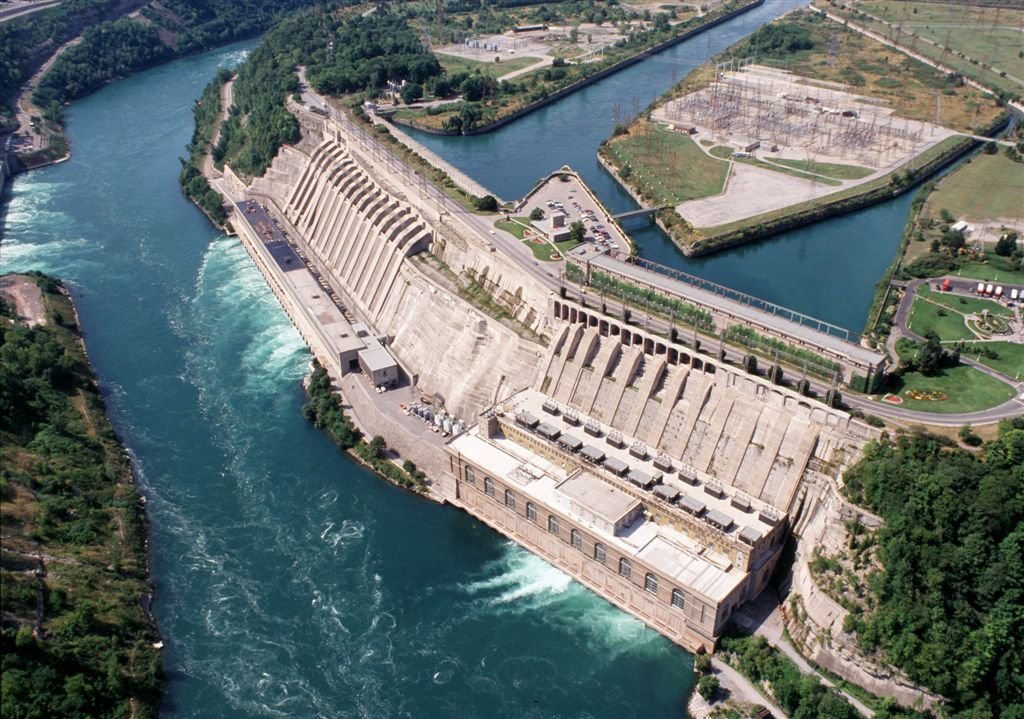
\includegraphics[width=\textwidth]{figures/adam_beck_complex.jpg}
	\caption{Sir Adam Beck Hydroelectric Generating Stations \citep{adam_back_complex}}
	\label{fig:power_plant}
\end{figure}

\subsection{Busses}
The most basic mathematical description of a an electric circuit, which an power net is, would be through admittances $Y_{ik}$ between the nodes $i$ and $k$, node voltages $U_k$ and branch currents $I_k$. In this case the element-based formulation
\begin{equation}
	\sum_i Y_{ik} U_i = I_k,
	\label{eq:current_controlled}
\end{equation}
will be used. If the loads and inputs would be current-controlled we could already stop at this point, solve the equation system and receive the node voltages as result. Unfortunately, most elements in a power net are defined through power, which is fed in, and load, which is drawn from the power net. Therefore, we have to extend \neweqref{current_controlled} with a term for a constant power $S_k = P_k + j Q_k = U_k I_k^\star$ at the node $k$ and receive
\begin{equation}
	\sum_i Y_{ik} U_i = I_k + \frac{S_j^\star}{U_j^\star}.
	\label{eq:pq_bus}
\end{equation}
This formula is already the definition of a so-called PQ-bus, as at the node the real and reactive power is the defined.
Another type of bus is a slack bus. At this bus the voltage is defined, therefore we do not need any further description of this bus, but the bus is also part from neighbour busses through the branch currents $Y_{ik} U_i$. In this case, if one of the branch currents is already known, this value can be moved to the right hand side of the equation \neweqref{pq_bus} and combined with $I_k$. Although, slack busses show up only in the constant currents of the right hand sides, there must be always at least one slack bus in the power net, as this bus then defines the rotation of the system and compensates mismatches in the total power sum. In practice, typically a major power plant is selected as slack bus.
The third important type of bus, beside the slack bus and PQ-bus, is the PV-bus. This is already some sort of control, as at such a node the real power $P_k$ and the voltage magnitude $|U_k|$ is defined. The implementation of this bus type depends on the algorithm which is used to calculate the missing node voltages, therefore I will discuss this in the section about the algorithms.

\subsection{Admittance Matrix}
The admittance matrix $\mat Y = (Y_{ik})$ is filled with the admittances between the nodes. More complex elements, like controlled sources, actually have to be voltage controlled, so that they can be modelled with an admittance matrix. Fortunately, most elements, which are not voltage controlled, can be transformed through a gyrator, which itself can be modelled through voltage controlled elements.

As during the modelling later several kinds of electric elements are used I will describe for each of them how they effect the admittance matrix. Each circuit element is there defined through a partial admittance matrix $\mat Y_p$, which have to be summed up afterwards to get the total admittance matrix $\mat Y$:
\begin{equation}
	\mat Y = \sum_i \mat Y_{p,i}
\end{equation}

The same superposition applies also for the current sources, if there are any.
\begin{equation}
	\vec I = \sum_i \vec I_{p,i}
\end{equation}

The two most important elements are the admittance, which is part of nearly every model of a net element, and the ideal transformer, which is mainly used for modelling real transformers which non-nominal ratios. The controlled source and the gyrator are actually only used to model the ideal transformer, which is build upon these elements.

\subsubsection{Admittance}

\begin{figure}
	\centering
	\begin{circuitikz}
	\draw (0, 0) node[left] {$U_\alpha$} to [R=$G$,o-o] (3, 0) node[right] {$U_\beta$};
\end{circuitikz} 

	\caption{Admittance $G$ between the nodes $\alpha$ and $\beta$}
	\label{fig:admittance}
\end{figure}

The admittance $G$ between the nodes $\alpha$ and $\beta$ \figref{admittance} causes the currents
\begin{equation}
	I_\alpha = (U_{k,\alpha} - U_{k,\beta}) G
\end{equation}
and
\begin{equation}
	I_\beta = (U_{k,\beta} - U_{k,\alpha}) G,
\end{equation}
which have to be considered in the admittance matrix through
\begin{equation}
	\mat Y_p = 	
	\begin{blockarray}{cccccc}
		\begin{block}{[ccccc]c}
		 		& \vdots	&			& \vdots	&			& \\
		\cdots	& G			& \cdots	& -G		& \cdots	& \alpha \\
		 		& \vdots	&			& \vdots	&			& \\
		\cdots	& -G		& \cdots	& G			& \cdots	& \beta \\
		 		& \vdots	&			& \vdots	&			& \\
		\end{block}
				& \alpha	&			& \beta		&			& 
	\end{blockarray}
\end{equation}

\subsubsection{Voltage Controlled Current Source}

\begin{figure}
	\centering
	\begin{circuitikz}
	\draw (0, 0) node[left] {$U_\delta$} to[open,o-o,v^=$u_{in}$] (0, 4) node[left] {$U_\gamma$};
	\draw (3, 4) to[european controlled current source,i=$g_m u_{in}$] (3, 0);
	\draw (3, 4) to[short,-o] (4, 4) node[right] {$U_\alpha$};
	\draw (3, 0) to[short,-o] (4, 0) node[right] {$U_\beta$};
\end{circuitikz} 

	\caption{Voltage controlled current source}
	\label{fig:voltage_controlled_current_source}
\end{figure}

The voltage controlled current source (VCCS) is again defined through the two branch currents
\begin{equation}
	I_\alpha = (U_{k,\gamma} - U_{k,\delta}) g_m
\end{equation}
and
\begin{equation}
	I_\beta = (U_{k,\delta} - U_{k,\gamma}) g_m,
\end{equation}
but with the difference to the admittance that this time the current is controlled by different nodes.

\begin{equation}
	\mat Y_p = 	
	\begin{blockarray}{cccccc}
		\begin{block}{[ccccc]c}
		 		& \vdots	&			& \vdots	&			& \\
		\cdots	& g_m		& \cdots	& -g_m		& \cdots	& \alpha \\
		 		& \vdots	&			& \vdots	&			& \\
		\cdots	& -g_m		& \cdots	& g_m		& \cdots	& \beta \\
		 		& \vdots	&			& \vdots	&			& \\
		\end{block}
				& \gamma	&			& \delta	&			& 
	\end{blockarray}
\end{equation}

\subsubsection{Gyrator}

\begin{figure}
	\centering
	\begin{circuitikz}
	\draw (0, 0) node[gyrator] (G) {};
	\draw (G.base) node{$G_D$};
  	\draw ($(G.A1) - (1, 0)$) node[left] {$U_\alpha$} to[short,o-,i=$i_1$] (G.A1);
  	\draw (G.A2) to[short,-o] ($(G.A2) - (1, 0)$) node[left] {$U_\beta$};
  	\draw ($(G.B1) + (1, 0)$) node[right] {$U_\gamma$} to[short,o-,i=$i_2$] (G.B1);
  	\draw (G.B2) to[short,-o] ($(G.B2) + (1, 0)$) node[right] {$U_\delta$};
  	\draw ($(G.A2) - (1, 0)$) to[open,v^=$u_1$] ($(G.A1) - (1, 0)$);
  	\draw ($(G.B2) + (1, 0)$) to[open,v=$u_2$] ($(G.B1) + (1, 0)$);
\end{circuitikz}
	\caption{Gyrator}
	\label{fig:gyrator_original}
\end{figure}

\begin{figure}
	\centering
	\begin{circuitikz}	
	\draw (1, 2.5) to[european controlled current source,i_=$G_D u_2$] (1, 0);
	\draw (-1, 2.5) node[left] {$U_\alpha$} to[short,i=$i_1$,o-] (1, 2.5);
	\draw (1, 0) to[short,-o] (-1, 0) node[left] {$U_\beta$};
	\draw (-1, 0) to[open,v^=$u_1$] (-1, 2.5);
	\draw (3, 2.5) to[european controlled current source,i=$-G_D u_1$] (3, 0);
	\draw (5, 2.5) node[right] {$U_\gamma$} to[short,i=$i_2$,o-] (3, 2.5);
	\draw (3, 0) to[short,-o] (5, 0) node[right] {$U_\delta$};
	\draw (5, 0) to[open,v=$u_2$] (5, 2.5);
\end{circuitikz} 

	\caption{Equivalent circuit for a gyrator}
	\label{fig:gyrator_equivalent}
\end{figure}

The gyrator \figref{gyrator_original}, which is defined by
\begin{equation}
	i_1 = G_D u_2
\end{equation}
and
\begin{equation}
	i_2 = -G_D u_1
\end{equation}
can be replaced with two VCCSs like in \figref{gyrator_equivalent}.

\subsubsection{Ideal Transformer}

\begin{figure}
	\centering
	\begin{circuitikz}
	\draw (0, 0) node[transformer core] (T) {};
	\draw ($(T.base) + (0, 0.3)$) node{$a : 1$};
  	\draw ($(T.A1) - (1, 0)$) node[left] {$U_\alpha$} to[short,o-,i=$i_1$] (T.A1);
  	\draw (T.A2) to[short,-o] ($(T.A2) - (1, 0)$) node[left] {$U_\beta$};
  	\draw ($(T.B1) + (1, 0)$) node[right] {$U_\gamma$} to[short,o-,i=$i_2$] (T.B1);
  	\draw (T.B2) to[short,-o] ($(T.B2) + (1, 0)$) node[right] {$U_\delta$};
  	\draw ($(T.A2) - (1, 0)$) to[open,v^=$u_1$] ($(T.A1) - (1, 0)$);
  	\draw ($(T.B2) + (1, 0)$) to[open,v=$u_2$] ($(T.B1) + (1, 0)$);
\end{circuitikz}
	\caption{Ideal transformer}
	\label{fig:ideal_transformer_original}
\end{figure}

\begin{figure}
	\centering
	\begin{circuitikz}
	\draw (0, 0) node[gyrator] (G1) {};
	\draw (2, 0) node[gyrator] (G2) {};
	\draw (G1.base) node{$a R$};
	\draw (G2.base) node{$R$};
	\draw (G1.B1) to[short,-*] (G1.B1) node[above] {$U_\epsilon$};
  	\draw ($(G1.A1) - (0.5, 0)$) node[left] {$U_\alpha$} to[short,o-,i=$i_1$] (G1.A1);
  	\draw (G1.A2) to[short,-o] ($(G1.A2) - (0.5, 0)$) node[left] {$U_\beta$};
  	\draw ($(G2.B1) + (0.5, 0)$) node[right] {$U_\gamma$} to[short,o-,i=$i_2$] (G2.B1);
  	\draw (G2.B2) to[short,-o] ($(G2.B2) + (0.5, 0)$) node[right] {$U_\delta$};
  	\draw ($(G1.A2) - (0.5, 0)$) to[open,v^=$u_1$] ($(G1.A1) - (0.5, 0)$);
  	\draw ($(G2.B2) + (0.5, 0)$) to[open,v=$u_2$] ($(G2.B1) + (0.5, 0)$);
  	\draw (G1.A2) to[short] (G1.B2);
\end{circuitikz}
	\caption{Equivalent circuit for an ideal transformer}
	\label{fig:ideal_transformer_equivalent}
\end{figure}

An ideal transformer like in \figref{ideal_transformer_original} is modelled with two gyrators according to the circuit \figref{ideal_transformer_equivalent}. The gyrators themselves have to be replaced by voltage controlled elements, like it was presented previously.

The parameter $R$ in this model can be chosen freely in theory, but for numerical reasons I recommend such a scaling of the internal node, that it is in the range of the nominal voltages. To be able to do this an estimation of the load flow over the transformer is needed, but it is sufficient to have a very rough estimate. If the scaling is chosen improperly especially the iterative methods to solve the load flow problem will not convergence in most cases.

\section{Modelling of Net Elements}

The power net elements are modelled through admittances and busses, therefore we will use the previously derived knowledge to describe the behaviour of the net elements.

All external nodes which exist in a power net are by default PQ-busses with no load, therefore $P = 0$ and $Q = 0$. The direct combination of PQ-busses leads to a summation of the partial inputs (or loads, depending on the sign). The direct connection of a PV-bus to a PQ-bus instead has the result, that bus is forced to become a PV-bus with the values $P_{total} = P_{PV} + P_{PQ}$ and $V_{total} = V_{PV}$. The reactive power of the PQ-node is assumed to be provided by the PV-bus. The third type of busses, a slack bus, can be combined with a PQ-bus too. In this case all loads are provided by the slack bus itself, therefore the total result is a slack bus.

As it would lead to an overspecified problem PV-busses must not be connected to slack busses. Theoretically this is possible if the PV-bus has the same voltage magnitude as the slack bus, but in practice this case does not occur and can be neglected.

\subsection{Transmission Line}
A transmission line is modelled only with admittances like in \figref{transmission_line}. The values $Y_q$ and $Y_l$ can be derived from the wave impedance $Z_W$, the propagation constant $\gamma$ and the length of the transmission line through
\begin{equation}
	Y_l = \frac{1}{Z_W \sinh \left( \gamma l \right)}
\end{equation}
and
\begin{equation}
	\frac{Y_q}{2} = \frac{1}{Z_W} \tanh \left( \frac{\gamma l}{2} \right),
\end{equation}
as shown in \citep[p. 155]{powerSystemAnalysis}. The wave impedance and the propagation constant can be calculated from the electrical characteristics with
\begin{equation}
	Z_W = \sqrt{\frac{R' + j \omega L'}{G' + j \omega C}}
\end{equation}
and 
\begin{equation}
	\gamma = \sqrt{\left( R' + j \omega L' \right) \left( G' + j \omega C \right)},
\end{equation}
also derived in \citep[p. 153]{powerSystemAnalysis}.

\begin{figure}
	\centering
	\begin{circuitikz}
	\draw (1, 0) to [R=$\frac{Y_{q}}{2}$,*-*] (1, 2.5);
	\draw (1, 2.5) to [R=$Y_{l}$,*-*] (3.5, 2.5);
	\draw (3.5, 0) to [R=$\frac{Y_{q}}{2}$,*-*] (3.5, 2.5);
	\draw (1, 0) to (3.5, 0);
	\draw (0, 0) to [short,o-*] (1, 0);
	\draw (0, 2.5) to [short,o-*] (1, 2.5);
	\draw (3.5, 0) to [short,*-o] (4.5, 0);
	\draw (3.5, 2.5) to [short,*-o] (4.5, 2.5);
	\draw (1, 0) to (1, -0.25) node[ground] {};
	\draw (0, 0) to [open,v^=$U_i$] (0, 2.5);
	\draw (4.5, 0) to [open,v=$U_j$] (4.5, 2.5);
\end{circuitikz} 

	\caption{Equivalent circuit for a transmission line}
	\label{fig:transmission_line}
\end{figure}

\subsection{Load}
A load can be modelled through a PQ-bus and no change to the admittance matrix. If there are several loads connected to one node their values sum up as already discussed before.

\subsection{Generator}

\begin{figure}
	\centering
	\begin{circuitikz}
	\draw (0, 0) node[below] {$|U| = E$, $P = P_{in}$} to [R=$jX_d$,*-o] (4, 0) node[above] {$U_\alpha$};
\end{circuitikz} 

	\caption{Equivalent circuit for a generator}
	\label{fig:generator}
\end{figure}

Generators are represented through an synchronous reactance $X_d$, which models internal losses, and a PV-bus, like it can be seen in \figref{generator}. The voltage magnitude at the internal PV-bus is the excitation voltage $E$ and the real power input is determined by the mechanical power and some transformation losses. 

If the synchronous reactance is not zero the external node $\alpha$ is not forced to any certain bus type, but if it is zero, the bus is forced to become a PV-bus.

\subsection{Transformer}

\subsection{Feed-In}

\section{Calculation Methods}

\subsection{Classification of Methods}

\subsection{Current Iteration}
\label{sec:current_iteration}

\subsection{Newton-Raphson}
\label{sec:newton_raphson}

\subsection{Fast-decoupled-load-flow}
\label{sec:fdlf}

\subsection{Holomorphic Embedding Load Flow}
\label{sec:helm}

\subsubsection{Calculation of Coefficients}

\paragraph{Slack-Busses}

\paragraph{PQ-Busses}

\paragraph{PV-Busses}

\subsubsection{Analytic Continuation with Wynn's Epsilon Method}
